\documentclass{beamer}

% Modern, minimal beamer theme
\usetheme[progressbar=frametitle, numbering=fraction, block=fill]{metropolis}
\usecolortheme{metropolis}
\definecolor{myblue}{HTML}{005F73}
\definecolor{mygreen}{HTML}{94D2BD}
\definecolor{mygray}{HTML}{E9ECEF}
\setbeamercolor{frametitle}{bg=myblue, fg=white}
\setbeamercolor{title}{fg=myblue}
\setbeamercolor{structure}{fg=myblue}
\setbeamercolor{block title}{bg=myblue, fg=white}
\setbeamercolor{block body}{bg=mygray, fg=black}
\setbeamercolor{item}{fg=myblue}
\setbeamercolor{enumerate item}{fg=myblue}

\usepackage{graphicx}
\usepackage{verbatim}
\usepackage[T1]{fontenc}
\usepackage[utf8]{inputenc}
\usepackage[spanish]{babel}
\usepackage{hyperref}
\usepackage{listings}
\usepackage{listingsutf8}
\usepackage{xcolor}

% Configuración de resaltado SQL
\lstdefinelanguage{SQL}{
  morekeywords={
    select,from,where,join,inner,left,right,full,on,group,by,having,order,asc,desc,
    limit,offset,union,all,distinct,insert,into,values,update,set,delete,create,table,
    primary,key,foreign,not,null,default,alter,add,drop,constraint,and,or,as,like,in,between
  },
  sensitive=false
}

\lstset{
  language=SQL,
  basicstyle=\ttfamily\small,
  keywordstyle=\color{myblue}\bfseries,
  stringstyle=\color{red!70!black},
  commentstyle=\color{gray},
  columns=fullflexible,
  keepspaces=true,
  showstringspaces=false,
  inputencoding=utf8,
  extendedchars=true,
  backgroundcolor=\color{mygray},
  frame=single,
  rulecolor=\color{myblue},
  literate={á}{{\'a}}1 {é}{{\'e}}1 {í}{{\'\i}}1 {ó}{{\'o}}1 {ú}{{\'u}}1
           {Á}{{\'A}}1 {É}{{\'E}}1 {Í}{{\'I}}1 {Ó}{{\'O}}1 {Ú}{{\'U}}1
           {ñ}{{\~n}}1 {Ñ}{{\~N}}1 {ü}{{\"u}}1 {Ü}{{\"U}}1
}

\title{Introducción a las Bases de Datos}
\author{Profesor: Víctor de Juan}
\date{\today}

\begin{document}
% ============================
% ========== SLIDE ===========
% ============================

% Portada
\begin{frame}
  \titlepage
\end{frame}

% ============================
% ========== SLIDE ===========
% ============================
% Diapositiva 1: Introducción al supuesto práctico
\begin{frame}
  \frametitle{Supuesto Práctico: Tienda Online}
Una pequeña empresa quiere poner en marcha una tienda online para vender sus productos a través de Internet.
Para gestionar su actividad, necesita almacenar información básica sobre los clientes que se registran
(sus datos de contacto y país de residencia), así como el catálogo de productos que ofrece, con sus precios y
las unidades disponibles en stock.
%
Además, debe guardar un historial de los pedidos que hacen los clientes,
cada uno con sus correspondientes artículos, cantidades y el precio aplicado en el momento de la compra.
%
Por otro lado, la empresa quiere llevar un control de los pagos asociados a cada pedido, de modo que pueda registrar la fecha,
el importe abonado y el método de pago utilizado (tarjeta, transferencia o PayPal).

\end{frame}

% ============================
% ========== SLIDE ===========
% ============================

% Diapositiva 2: Solución: Diagrama Entidad-Relación
\begin{frame}
  \frametitle{Solución}

  \begin{center}
   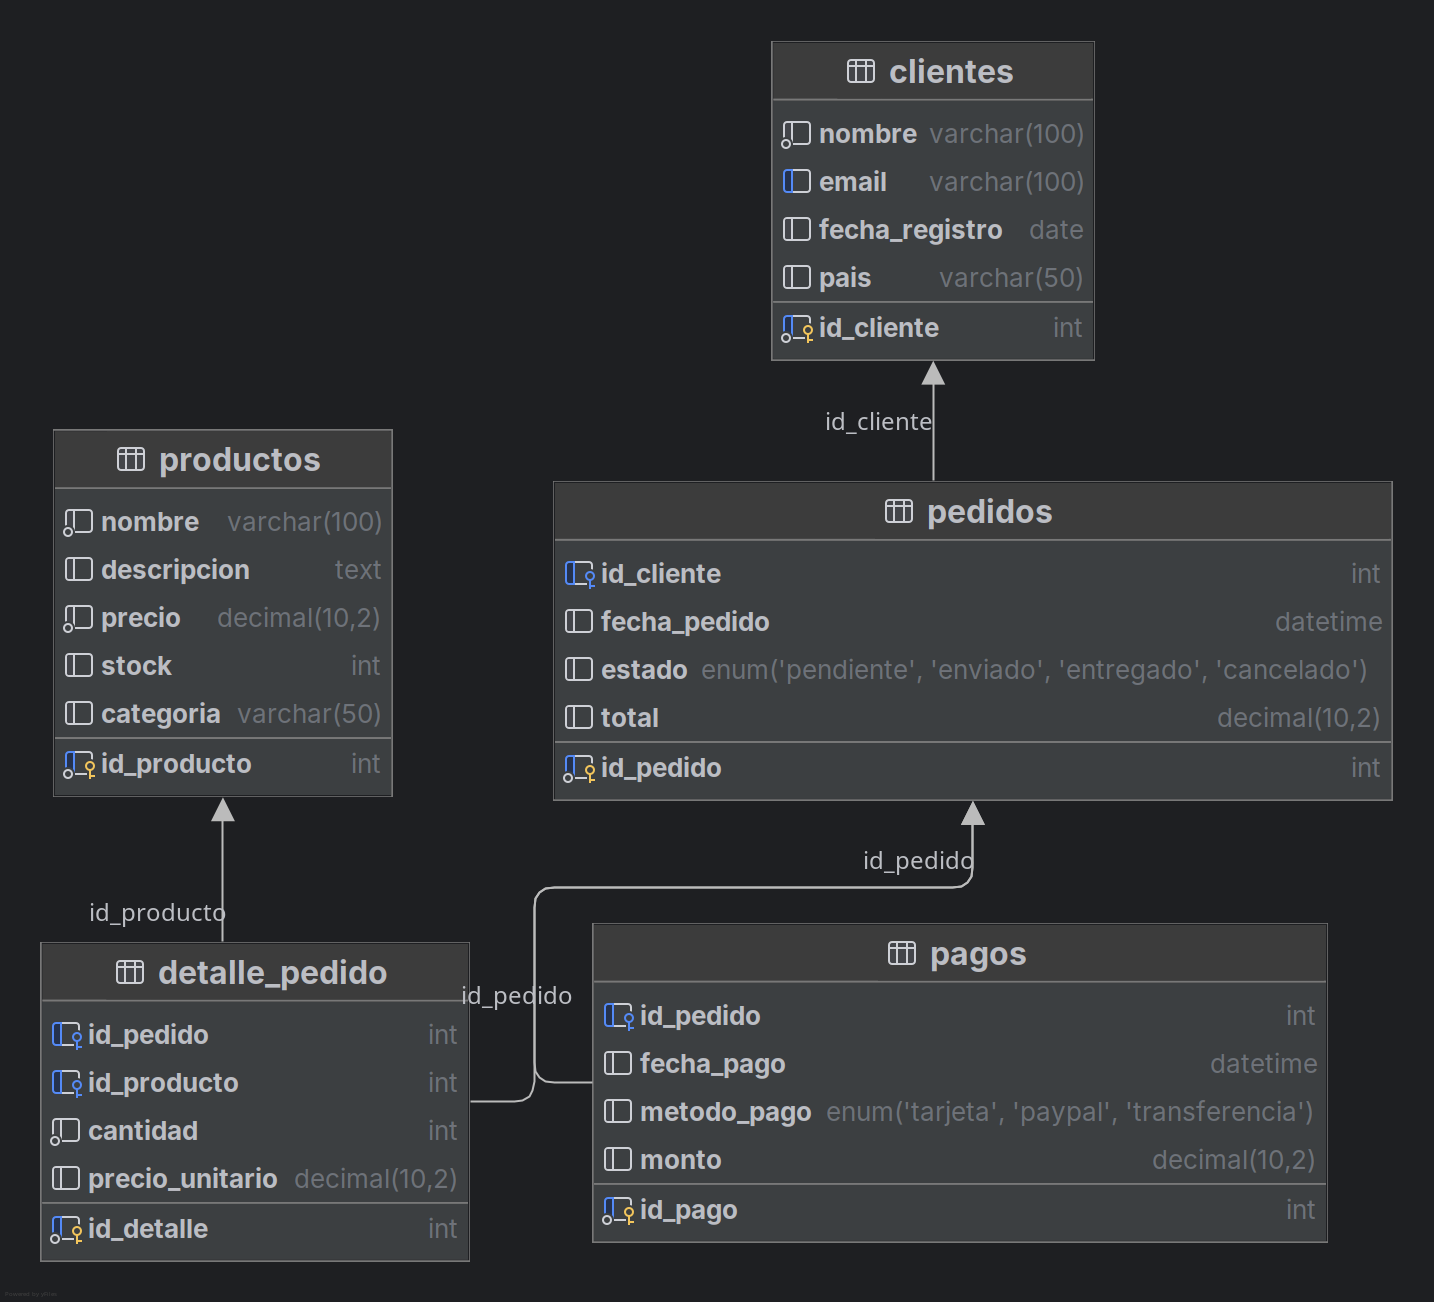
\includegraphics[width=0.6\textwidth]{../../dbs/tiendaonline/tiendaonline-ER} % Aquí insertas el diagrama ER que hayas generado con tiendaonline-schema.sql
  \end{center}

  Este es el modelo que utilizaremos como solución.
  Cada rectángulo es una entidad (tabla), y las líneas representan las relaciones entre ellas.
  Más detalles de cómo se conectan vendrán más adelante.

\end{frame}

% ============================
% ========== SLIDE ===========
% ============================

% Diapositiva 3: Presentación de los datos
\begin{frame}  \frametitle{Presentación de los Datos}

	Ver \href{https://github.com/Dpto-Informatica-IES-Francisco-de-Goya/BasesDeDatos/blob/main/dbs/tiendaonline/tienda\_online\_full\_data.md}{github}.
\end{frame}

% ============================
% ========== SLIDE ===========
% ============================

% Diapositiva 4: Preguntas a resolver con consultas
\begin{frame}[fragile]
  \frametitle{Preguntas:}

  A partir de los datos que tenemos, vamos a plantear algunas preguntas:

  \begin{enumerate}
    \item ¿Qué productos tiene más stock?
    \item ¿Cuántos clientes hay en España?
    \item ¿Qué productos ha comprado Ana?
    \item ¿Cuánto ha pagado Ana?
    \item ¿Cuántos pagos han sido realizados con tarjeta?


  \end{enumerate}
\end{frame}

% ============================
% ========== SLIDE ===========
% ============================



\begin{frame}[fragile]
  \frametitle{Soluciones SQL (1/2):}

  \begin{enumerate}
    \item ¿Qué productos tiene más stock?
    \begin{lstlisting}
select * from productos order by stock limit 1;
    \end{lstlisting}

    \item ¿Cuántos clientes hay en España?
    \begin{lstlisting}
select * from clientes where pais="España";
    \end{lstlisting}

    \item ¿Qué productos ha comprado Ana?
    \begin{lstlisting}
select *
from productos
join detalle_pedido using(id_producto)
join pedidos using(id_pedido)
join clientes using(id_cliente)
where clientes.nombre like "Ana%";
    \end{lstlisting}
  \end{enumerate}
\end{frame}

\begin{frame}[fragile]
  \frametitle{Soluciones SQL (2/2):}

  Continuamos con las preguntas:

  \begin{enumerate}
    \setcounter{enumi}{3}
    \item ¿Cuánto ha pagado Ana?
    \begin{lstlisting}
select id_cliente, sum(precio_unitario * cantidad)
from productos
  join detalle_pedido using(id_producto)
  join pedidos using(id_pedido)
  join clientes using(id_cliente)
where clientes.nombre like "Ana%"
group by id_cliente;
    \end{lstlisting}

    \item ¿Cuántos pagos han sido realizados con tarjeta?
    \begin{lstlisting}
select count(id_pago) from pagos 
  where metodo_pago = "tarjeta";
    \end{lstlisting}
  \end{enumerate}
\end{frame}

% ============================
% ========== SLIDE ===========
% ============================


\begin{frame}[fragile]
  \frametitle{Preparando el entorno: Descarga y carga de la base de datos}

  \begin{enumerate}
    \item Abre una terminal en tu sistema operativo (por ejemplo, con \texttt{CTRL+ALT+T} en Linux).
    \item Descarga los archivos \texttt{tiendaonline-schema.sql} y \texttt{tiendaonline-data.sql} desde el repositorio de GitHub y colócalos en el mismo directorio donde vas a trabajar.
    \item Accede a MySQL con tu usuario y contraseña. Por ejemplo:
    \begin{lstlisting}[language=bash, backgroundcolor=\color{gray!10}]
$ mysql -u tu_usuario -p
    \end{lstlisting}
    \item Comprueba las bases de datos existentes:
    \begin{lstlisting}[language=SQL, backgroundcolor=\color{gray!10}]
show databases;
    \end{lstlisting}
  \end{enumerate}
\end{frame}

\begin{frame}[fragile]
  \frametitle{Preparando el entorno: Cargar estructura y datos}

  \begin{enumerate}
    \setcounter{enumi}{4}
    \item Carga la estructura de la base de datos ejecutando:
    \begin{lstlisting}[language=SQL, backgroundcolor=\color{gray!10}]
source tiendaonline-schema.sql
    \end{lstlisting}
    \item Carga los datos en la base de datos:
    \begin{lstlisting}[language=SQL, backgroundcolor=\color{gray!10}]
source tiendaonline-data.sql
    \end{lstlisting}
    \item Comprueba que los datos se han cargado correctamente, por ejemplo:
    \begin{lstlisting}[language=SQL, backgroundcolor=\color{gray!10}]
show tables;
select * from productos limit 5;
    \end{lstlisting}
    \item Ahora puedes probar las consultas SQL vistas en las diapositivas anteriores.
  \end{enumerate}
\end{frame}

% ============================
% ========== SLIDE ===========
% ============================

% Diapositiva final: Tarea
\begin{frame}
  \frametitle{Tarea}

  \textbf{Entrega:} Tendrás que realizar varias capturas de pantalla en las que se vea cómo has ejecutado todas las consultas SQL mostradas como ejemplo en las diapositivas anteriores. Estas capturas se entregarán en la tarea del aula virtual.\\[1em]
  \begin{itemize}
    \item Las capturas deben mostrar la terminal o herramienta que haya utilizado para ejecutar las consultas.
    \item Asegúrese de que se vean claramente tanto las consultas como los resultados obtenidos.
    \item Adjunte todas las imágenes en la tarea correspondiente del aula virtual.
  \end{itemize}

\end{frame}

\end{document}
